\documentclass[letter,11pt]{article}

\usepackage[spanish,es-nodecimaldot]{babel}
\usepackage[utf8]{inputenc}

\usepackage{lmodern}
\usepackage[T1]{fontenc}
\usepackage{textcomp}

\usepackage{framed}
\usepackage[svgnames]{xcolor}
\colorlet{shadecolor}{Gainsboro!50}

\usepackage{enumitem}
\usepackage{graphicx}
\usepackage{pstricks}

\usepackage{anysize}
\marginsize{3cm}{2cm}{2cm}{3cm}

\usepackage{siunitx}
\usepackage{amsmath}
\usepackage{array}
\usepackage{alltt}

\usepackage{fancyhdr}
\usepackage{lastpage}
\pagestyle{fancy}
\fancyhf{}
\fancyhead[LE,RO]{Física Básica II}
\fancyfoot[CO,CE]{\thepage\ de \pageref{LastPage}}

\special{papersize=215.9mm,279.4mm}

\usepackage[
    pdfauthor={Carlos Eduardo Caballero Burgoa},%
    pdftitle={Física Básica II},%
    pdfsubject={Tarea 11},%
    colorlinks,%
    citecolor=black,%
    filecolor=black,%
    linkcolor=black,%
    urlcolor=black,
    breaklinks]{hyperref}
\usepackage{breakurl}

\newcommand{\blankpage}{
\newpage
\thispagestyle{empty}
\mbox{}
\newpage
}

\renewcommand{\arraystretch}{1.2}

\begin{document}

\begin{center}
    {\Large \bf{Tarea \#11}}
\end{center}

\section{Ejercicio 1}
Calcule el centro de masa del siguiente sistema de distribución superficial
uniforme. \emph{Sugerencia}: Utilice un diferencial de área apropiado.

\begin{figure}[!h]
\centering
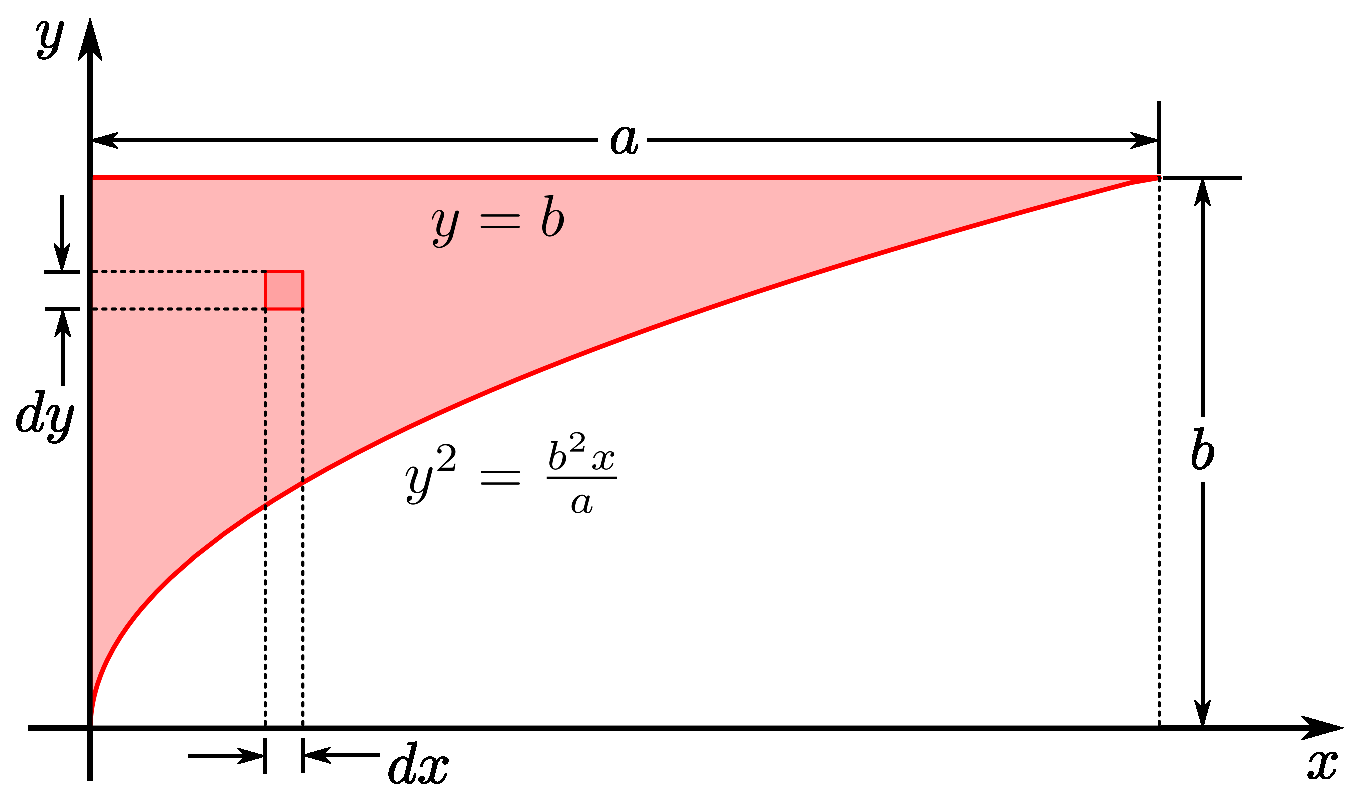
\includegraphics[scale=0.45]{resources/f1.eps}
\end{figure}

\textbf{Solución:} \\

Dada la ecuación del centro de masa:

\begin{equation}
    \vec{r}_{cm} = \frac{1}{M} \int_{M} \vec{r} \cdot dm
\label{base1}
\end{equation}

Y considerando la distribución homogénea de la masa sobre el material:
\begin{equation*}
    \sigma = \frac{dm}{ds} = ctte
\end{equation*}

Por tanto:
\begin{equation}
    dm = \sigma \cdot ds = \sigma \cdot dx \cdot dy
\label{dm1}
\end{equation}

Reemplazando (\ref{dm1}) en (\ref{base1}):
\begin{equation*}
    \vec{r}_{cm} = \frac{1}{M} \int_{0}^{M} \vec{r} \cdot \sigma \cdot ds
\end{equation*}

Reemplazando $\vec{r}$ por sus componentes:
\begin{equation*}
    \vec{r}_{cm} = \frac{1}{M} \int_{0}^{S} (x \hat{i} + y \hat{j}) \cdot \sigma \cdot ds = \frac{\sigma}{M} \int_{0}^{a} \int_{y_{min}}^{y_{max}} (x \hat{i} + y \hat{j}) \cdot dx \cdot dy
\end{equation*}

Sabiendo que los limites de la función son:
\begin{equation*}
    y_{min} = \sqrt{\frac{b^2 x}{a}}
\end{equation*}
\begin{equation*}
    y_{max} = b
\end{equation*}

Obtenemos la siguiente ecuación:
\begin{equation*}
    \vec{r}_{cm} = \frac{\sigma}{M} \int_{x = 0}^{x = a} \int_{y = \sqrt{\frac{b^2 x}{a}}}^{y = b} (x \hat{i} + y \hat{j}) \cdot dy \cdot dx
\end{equation*}

Para simplificar la resolución de la integral doble, se procede a cambiar el orden de integración, corrigiendo sus limites:
\begin{equation*}
    \vec{r}_{cm} = \frac{\sigma}{M} \int_{y = 0}^{y = b} \int_{x = 0}^{x = \frac{a y^2}{b^2}} (x \hat{i} + y \hat{j}) \cdot dx \cdot dy
\end{equation*}

Para $\hat{i}$:
\begin{equation*}
    x_{cm} = \frac{\sigma}{M} \int_{0}^{b} \int_{0}^{\frac{a y^2}{b^2}} x \cdot dx \cdot dy = \frac{\sigma}{M} \int_{0}^{b} \left(\int_{0}^{\frac{a y^2}{b^2}} x \cdot dx \right) dy = \frac{\sigma}{M} \int_{0}^{b} \frac{x^2}{2}\Biggr|_{0}^{\frac{a y^2}{b^2}} dy
\end{equation*}
\begin{equation*}
    x_{cm} = \frac{\sigma}{M} \int_{0}^{b} \left(\frac{a^2 y^4}{2 b^4} \right) dy = \frac{\sigma}{M} \frac{a^2}{2 b^4} \int_{0}^{b} y^4 dy
\end{equation*}
\begin{equation*}
    x_{cm} = \frac{\sigma}{M} \frac{a^2}{2 b^4} \frac{y^5}{5}\Biggr|_{0}^{b} = \frac{\sigma}{M} \left(\frac{a^2}{2 b^4} \frac{b^5}{5}\right) = \frac{\sigma}{M} \left(\frac{a^2 b}{10}\right)
\end{equation*}

Para $\hat{j}$:
\begin{equation*}
    y_{cm} = \frac{\sigma}{M} \int_{0}^{b} \int_{0}^{\frac{a y^2}{b^2}} y \cdot dx \cdot dy = \frac{\sigma}{M} \int_{0}^{b} y \left(\int_{0}^{\frac{a y^2}{b^2}} dx \right) dy = \frac{\sigma}{M} \int_{0}^{b} y \cdot x\Biggr|_{0}^{\frac{a y^2}{b^2}} dy
\end{equation*}
\begin{equation*}
    y_{cm} = \frac{\sigma}{M} \int_{0}^{b}  y \cdot \frac{a y^2}{b^2} dy = \frac{\sigma}{M} \frac{a}{b^2} \int_{0}^{b} y^3 dy
\end{equation*}
\begin{equation*}
    y_{cm} = \frac{\sigma}{M} \frac{a}{b^2} \frac{y^4}{4} \Biggr|_{0}^{b} = \frac{\sigma}{M} \left( \frac{a}{b^2} \frac{b^4}{4} \right) = \frac{\sigma}{M} \left( \frac{ab^2}{4} \right)
\end{equation*}

\vspace{0.5cm}
Uniendo ambas componentes:
\begin{equation}
    \vec{r}_{cm} = \frac{\sigma}{M} \left( \frac{a^2 b}{10} \right) \hat{i} + \frac{\sigma}{M} \left( \frac{a b^2}{4} \right) \hat{j}
\label{vector1}
\end{equation}

Integrando la ecuación (\ref{dm1}):
\begin{equation*}
    M = \sigma \int_{0}^{b} \int_{0}^{\frac{a y^2}{b^2}} dx \cdot dy = \sigma \int_{0}^{b} x\Biggr|_{0}^{\frac{a y^2}{b^2}} dy = \sigma \int_{0}^{b} \frac{a}{b^2} y^2 dy
\end{equation*}
\begin{equation*}
    M = \sigma \frac{a}{b^2} \int_{0}^{b} y^2 dy = \sigma \frac{a}{b^2} \frac{y^3}{3}\Biggr|_{0}^{b} = \sigma \frac{a}{b^2} \frac{b^3}{3} = \frac{\sigma}{3} a b
\end{equation*}

Reemplazando $M$ de la ecuación (\ref{vector1}), obtenemos:
\begin{equation*}
    \vec{r}_{cm} = \frac{3}{10} a \hat{i} + \frac{3}{4} b \hat{j}
\tag{resultado}
\end{equation*}

\section{Ejercicio 2}
Calcule el centro de masa del siguiente sistema de distribución superficial
uniforme. \emph{Sugerencia}: Utilice un diferencial de área apropiado.

\begin{figure}[!h]
\centering
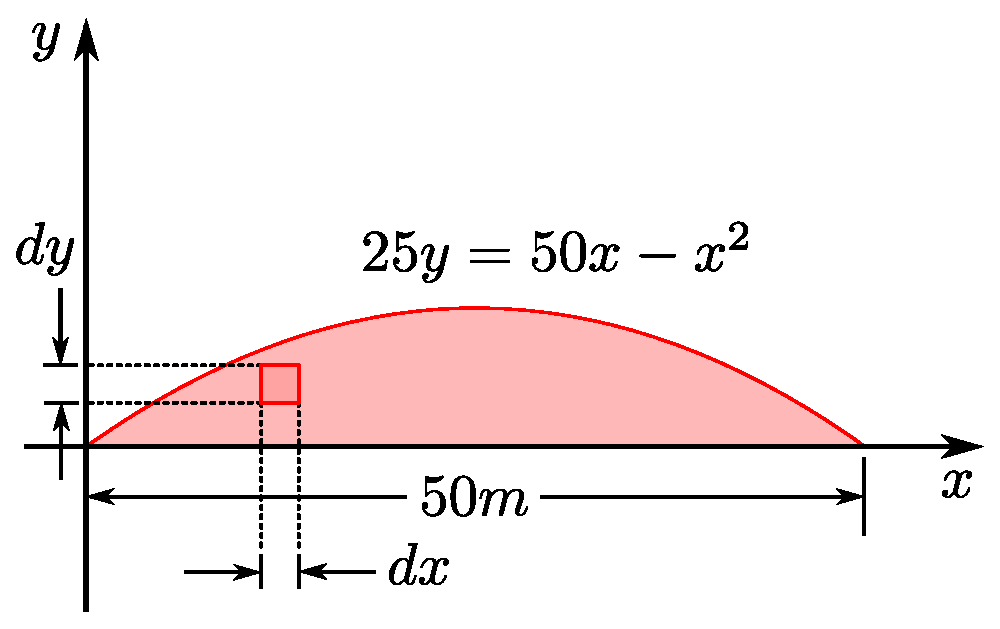
\includegraphics[scale=0.42]{resources/f2.eps}
\end{figure}

\textbf{Solución:} \\

Dada la ecuación del centro de masa:

\begin{equation}
    \vec{r}_{cm} = \frac{1}{M} \int_{M} \vec{r} \cdot dm
\label{base2}
\end{equation}

Y considerando la distribución homogénea de la masa sobre el material:
\begin{equation*}
    \sigma = \frac{dm}{ds} = ctte
\end{equation*}

Por tanto:
\begin{equation}
    dm = \sigma \cdot ds = \sigma \cdot dx \cdot dy
\label{dm2}
\end{equation}

Reemplazando (\ref{dm2}) en (\ref{base2}):
\begin{equation*}
    \vec{r}_{cm} = \frac{1}{M} \int_{0}^{M} \vec{r} \cdot \sigma \cdot ds
\end{equation*}

Reemplazando $\vec{r}$ por sus componentes:
\begin{equation*}
    \vec{r}_{cm} = \frac{1}{M} \int_{0}^{S} (x \hat{i} + y \hat{j}) \cdot \sigma \cdot ds = \frac{\sigma}{M} \int_{0}^{50} \int_{y_{min}}^{y_{max}} (x \hat{i} + y \hat{j}) \cdot dx \cdot dy
\end{equation*}

Sabiendo que los limites de la función son:
\begin{equation*}
    y_{min} = 0
\end{equation*}
\begin{equation*}
    y_{max} = \frac{50x - x^2}{25}
\end{equation*}

Obtenemos la siguiente ecuación:
\begin{equation*}
    \vec{r}_{cm} = \frac{\sigma}{M} \int_{x = 0}^{x = 50} \int_{y = 0}^{y = \frac{50x - x^2}{25}} (x \hat{i} + y \hat{j}) \cdot dy \cdot dx
\end{equation*}

Para $\hat{i}$:
\begin{equation*}
    x_{cm} = \frac{\sigma}{M} \int_{0}^{50} \int_{0}^{\frac{50x - x^2}{25}} x \cdot dy \cdot dx = \frac{\sigma}{M} \int_{0}^{50} x \cdot \left(\int_{0}^{\frac{50x - x^2}{25}} dy \right) dx = \frac{\sigma}{M} \int_{0}^{50} x \cdot y\Biggr|_{0}^{\frac{50x - x^2}{25}} dx
\end{equation*}
\begin{equation*}
    x_{cm} = \frac{\sigma}{M} \int_{0}^{50} x \left(\frac{50x - x^2}{25} \right) dx = \frac{\sigma}{M} \frac{1}{25} \int_{0}^{50} (50x^2 - x^3) \cdot dx = \frac{\sigma}{M} \frac{1}{25} \left(\frac{50x^3}{3} - \frac{x^4}{4}\right)\Biggr|_{0}^{50}
\end{equation*}
\begin{equation*}
    x_{cm} = \frac{\sigma}{M} \frac{1}{25} 50^4 \left(\frac{1}{3} - \frac{1}{4}\right) = \frac{\sigma}{M}\frac{1}{25}\frac{50^4}{12} = \frac{\sigma}{M} \frac{50^4}{300}
\end{equation*}

Para $\hat{j}$:
\begin{equation*}
    y_{cm} = \frac{\sigma}{M} \int_{0}^{50} \int_{0}^{\frac{50x - x^2}{25}} y \cdot dy \cdot dx = \frac{\sigma}{M} \int_{0}^{50} \left(\int_{0}^{\frac{50x - x^2}{25}} y \cdot dy \right) dx = \frac{\sigma}{M} \int_{0}^{50} \frac{y^2}{2}\Biggr|_{0}^{\frac{50x - x^2}{25}} dx
\end{equation*}
\begin{equation*}
    y_{cm} = \frac{\sigma}{M} \int_{0}^{50} \left(\frac{1}{2} \left(\frac{50x - x^2}{25}\right)^2 \right) dx = \frac{\sigma}{M} \frac{1}{2} \frac{1}{25^2} \int_{0}^{50} (50^2 x^2 - 100 x^3 + x^4) \cdot dx
\end{equation*}
\begin{equation*}
    y_{cm} = \frac{\sigma}{M} \frac{1}{2} \frac{1}{25^2} \left(\frac{50^2 x^3}{3} - \frac{100 x^4}{4} + \frac{x^5}{5}\right)\Biggr|_{0}^{50} = \frac{\sigma}{M} \frac{1}{2} \frac{1}{25^2} \frac{50^5}{30} = \frac{\sigma}{M} \frac{50^5}{60 \cdot 25^2}
\end{equation*}

\vspace{0.5cm}
Uniendo ambas componentes:
\begin{equation}
    \vec{r}_{cm} = \frac{\sigma}{M} \left( \frac{50^4}{300} \right) \hat{i} + \frac{\sigma}{M} \left( \frac{50^5}{60 \cdot 25^2} \right) \hat{j}
\label{vector1}
\end{equation}

Integrando la ecuación (\ref{dm2}):
\begin{equation*}
    M = \sigma \int_{0}^{50} \int_{0}^{\frac{50x - x^2}{25}} dx \cdot dy = \sigma \int_{0}^{50} x\Biggr|_{0}^{\frac{50x - x^2}{25}} dy = \sigma \int_{0}^{50} \frac{50x - x^2}{25} dy
\end{equation*}
\begin{equation*}
    M = \frac{\sigma}{25} \int_{0}^{50} \left(\frac{50 x^2}{2} - \frac{x^3}{3}\right)\Biggr|_{0}^{50} = \frac{\sigma}{25} \frac{50^3}{6} = \frac{\sigma \cdot 50^3}{150}
\end{equation*}

Reemplazando $M$ de la ecuación (\ref{vector1}), obtenemos:
\begin{equation*}
    \vec{r}_{cm} = 25 \hat{i} + 10 \hat{j}
\tag{resultado}
\end{equation*}

\end{document}

